\documentclass[12pt, oneside]{amsart}
\usepackage{amsmath}
\usepackage{lipsum}
\linespread{1.25}
\setlength{\topmargin}{0.in}
\setlength{\oddsidemargin}{0.33in}
\setlength{\textheight}{9.0in}
\setlength{\textwidth}{6.0in}
%-------Packages---------
\usepackage{amssymb,amsfonts}
\usepackage[all,arc]{xy}
\usepackage{enumerate}
\usepackage{mathrsfs}
\usepackage{graphicx}
\usepackage{epstopdf}
\usepackage{listings}
\usepackage{appendix}
\usepackage{listings}
\usepackage{placeins}

%--------Theorem Environments--------
%theoremstyle{plain} --- default
\newtheorem{thm}{Theorem}[section]
\newtheorem{cor}[thm]{Corollary}
\newtheorem{prop}[thm]{Proposition}
\newtheorem{lem}[thm]{Lemma}
\newtheorem{conj}[thm]{Conjecture}
\newtheorem{quest}[thm]{Question}

\theoremstyle{definition}
\newtheorem{defn}[thm]{Definition}
\newtheorem{defns}[thm]{Definitions}
\newtheorem{con}[thm]{Construction}
\newtheorem{exmp}[thm]{Example}
\newtheorem{exmps}[thm]{Examples}
\newtheorem{notn}[thm]{Notation}
\newtheorem{notns}[thm]{Notations}
\newtheorem{addm}[thm]{Addendum}
\newtheorem{exer}[thm]{Exercise}

\theoremstyle{remark}
\newtheorem{rem}[thm]{Remark}
\newtheorem{rems}[thm]{Remarks}
\newtheorem{warn}[thm]{Warning}
\newtheorem{sch}[thm]{Scholium}
\newcommand{\be}{\begin{equation}}
\newcommand{\ee}{\end{equation}}
\makeatletter
\let\c@equation\c@thm
\makeatother
\numberwithin{equation}{section}

\usepackage[style=apa,sortcites=true,sorting=nyt,backend=biber,natbib=true]{biblatex}
%bibliographystyle{unsrtnat}
\addbibresource{Reference/reference.bib}
%%%%%%%%%%%%%%%%%%%%%%%%%%%%%%%%%%%%%%%%%%%%%%%%%%%%%%%%%%%%%%%%%%%%%%%%%%%%%%%%%
% your title/author/date information go here
%--------Meta Data: Fill in your info------


\title{On the Prediction-Powered Causal Inference}

\author{Xuan Li}

\date{December 23, 2024}

\begin{document}

\begin{abstract}
    This report serves as a qualifying paper for the UBC Statistics PhD program, providing a comprehensive summary of the paper Prediction-Powered Generalization of Causal Inference \citep{qp}. The original paper introduces a novel framework leveraging both randomized controlled trial (RCT) data and observational study (OS) data to estimate causal effects in a target population. Building on this foundation, we explore three extensions: (1) evaluating the framework's performance under covariate misrepresentation between the target and trial populations, (2) examining dynamically the bias-variance trade-off by analyzing how increasing RCT sample sizes affects the squared error of the average outcome estimators, and (3) proposing adaptive sampling strategies to optimize RCT participant selection. Through simulations, we demonstrate the strengths and limitations of the Prediction-Powered Causal Inference (PPCI) framework and assess the effectiveness of adaptive strategies in enhancing estimation accuracy while maintaining resource efficiency. These findings contribute to understanding the practical applicability of PPCI framework.
\end{abstract}
\maketitle
\tableofcontents

%%%%%%%%%%%%%%%%%%%%%%%%%%%%%%%%%%%%%%%%%%%%%%%%%%%%%%%%%%%%%%%%%%%%%%%%%%%%%%%%%section 1

\section{Introduction}
\subsection{Background}
Randomized controlled trials (RCTs) are the gold standard for causal inference, but are costly. They often fail to generalize to broader populations for various reasons, such as differences in effect modifiers, which can lead to confounding bias between the effects of the trial and the target population. This issue has prompted extensive research on integrating trial data with covariate information from the target population or with observational studies (OS). Previous works, such as \citep{Dahabreh2019}, \citep{Dahabreh2020}, and \citep{Bareinboim}, explored combining trial and OS data, while \citep{guo2021} and \citep{liao2023} investigated hybrid approaches to improve the estimate of the average treatment effect (ATE) and address confounding biases. \\

The original paper "Prediction-Powered Generalization of Causal Inference" advances this field by proposing a prediction-powered framework that combines RCT and OS data through machine learning models \citep{qp}. Unlike previous approaches, the framework flexibly defines the target population in a more general setting as trial-eligible individuals, separate from both trial and OS populations. The authors demonstrate that high-quality observational data can improve generalization even for small, unrepresentative trials, while maintaining robustness when observational data quality is low. 

\subsection{Our Extension}
Our study extends the Prediction-Powered Causal Inference (PPCI) framework with three key contributions. First, we evaluate the performance of the PPCI framework under a representational mismatch in covariate between the target and trial sets. In our experiment, while both sets are drawn from the same distribution, the trial set overrepresents higher values of the covariate, creating an imbalance. Second, we investigate the bias-variance trade-off by examining how increasing the RCT sample size affects the squared error (SE) in the average outcome estimates. Third, we introduce adaptive sampling strategies leveraging active learning to optimize RCT participant selection. This approach identifies the most informative samples to improve estimation accuracy while keeping the trial size constant. We employ three adaptive sampling strategies to refine the trial selection by selecting points with the greatest potential to reduce estimation error.

\section{Summary of the Original Paper}
\subsection{General Setting and Problem Definition}
The goal is to estimate the average potential outcome in a target population
\[
\mu_a := \mathbb{E}[Y^a \mid S = 0],
\]
which represents the mean potential outcome under treatment $A = a$ in the target population ($S = 0$). The dataset $D = \{W_i\}_{i=1}^n$ consists of:
\begin{itemize}
    \item $X$: Covariates, 
    \item $S \in \{0, 1, 2\}$: Population indicator ($S = 1$: trial, $S = 0$: target, $S = 2$: observational study),
    \item $A$: Treatment indicator ($A = 1$: treated, $A = 0$: untreated, in binary treatment setting),
    \item $Y$: Treatment outcome, with $Y^a$ represents the potential outcome under treatment $A = a$. In binary treatment setting, $Y^1$ represents the potential outcome when treated and $Y^0$ represents the potential outcome when untreated.
    \item $D_k$ is used to represent different datasets. We denote $D_0$ the target dataset with size $n_0 = \sum_{i=1}^n 1 \{S_i = 0\}$, $D_1$ the trial dataset with size $n_1 = \sum_{i=1}^n 1 \{S_i = 1\}$, $D$ the composite set consists $D_0$ and $D_1$ with size $n$, and $D_2$ the observational dataset with size $n_2$,
    \item $P$ represents the joint distribution of $W$. $P_1$ represents the trial population ($S = 1$) distribution, $P_0$ represents the target population ($S = 0$) distribution and $P_2$ represents the observational population ($S = 2$) distribution. For example, $X \sim P_0$ indicates a covariate drawn from the target population.
\end{itemize}


Notice that the original paper assumes a nested design, where the trial sample is drawn from a broader target population consisting of trial-eligible individuals. For non-participants ($S = 0$), only covariate data $X$ is available. For participants ($S = 1$) and observational samples ($S = 2$), treatment and outcome data ($A, Y$) are also observed. Observational data ($S = 2$) are from an external population, where treatment assignment $A$ could be biased (dependent on $X$ and possibly unobserved confounders). By utilizing trial data ($D_1$) and observational data ($D_2$), this set-up provides a framework for estimating causal effects in the target population ($D_0$). The main challenge lies in the lack of observed outcomes in the target population and potential biases in the observational data. Additionally, confounding by trial participation poses another challenge; however, this is addressed by our assumptions introduced later.\\

\subsection{Key Assumptions}
The identification of $\mu_a$ relies on the following five assumptions.
\textbf{Assumption 2.1 (Consistency)}: 
$A = a \implies Y = Y^a.
$
This assumption ensures the observed outcomes correspond to the potential outcomes being estimated. Without consistency, observed outcomes cannot be interpreted causally. For instance, if patients do not adhere to the treatment, their outcomes may not reflect the true treatment effect.\\

\textbf{Assumption 2.2 (Mean Ignorability of Treatment Assignment in Trial)}: 
$
\mathbb{E}[Y^a \mid X, S = 1] = \mathbb{E}[Y^a \mid X, S = 1, A = a].
$
In trials ($S = 1$), treatment assignment $A$ is independent of potential outcomes $Y^a$ given covariates $X$, a condition satisfied by randomization in RCTs.\\

\textbf{Assumption 2.3 (Positivity of Treatment Assignment in Trial)}:
$
P(A = a \mid X = x, S = 1) > 0.
$
For any covariate $X$ in the trial ($S = 1$), both treatment ($A = 1$) and control ($A = 0$) must have non-zero probabilities.\\

\textbf{Assumption 2.4 (Mean Ignorability of Trial Participation)}: 
$
\mathbb{E}[Y^a \mid X] = \mathbb{E}[Y^a \mid X, S = 1] = \mathbb{E}[Y^a \mid X, S = 0].
$
Given covariates $X$, potential outcomes $Y^a$ are the same on average for trial participants ($S = 1$) and non-participants ($S = 0$). This allows generalization of trial results to the target population by addressing covariate shifts between the two populations.\\

\textbf{Assumption 2.5 (Positivity of Selection Into Trial)}:
$
P(S = 0 \mid X = x) > 0 \implies P(S = 1 \mid X = x) > 0.
$
All individuals in the target population ($S = 0$) must have a non-zero chance of participating in the trial ($S = 1$), ensuring representation across all covariate levels so that we do not have to rely on pure extrapolation. \\


 Assumptions 2.1-2.3 are satisfied in RCT setting by design and enable causal inference within the trial sample ($S = 1$). Assumptions 2.4-2.5 are required for generalizing the causal effect from the trial sample ($S = 1$) to the broader target population ($S = 0$). Based on the assumptions, the identification formula for $\mu_a$ is defined as:
$$
\mu_a = \mathbb{E}_{X \sim P_0} [\mathbb{E}[Y^a \mid X, S = 0]]
= \mathbb{E}_{X \sim P_0} [\mathbb{E}[Y^a \mid X, S = 1]]
= \mathbb{E}_{X \sim P_0} [\mathbb{E}[Y \mid X, S = 1, A = a]].
$$
Note that $ \mu_a$ can be estimated using only covariate data from non-participants (\textit{S }= 0) and covariate, treatment, and outcome data from the trial participants (\textit{S }= 1). Besides approximating $\mu_a$ with the baseline estimator, the authors propose the \textbf{Prediction-Powered Causal Inference} framework, which introduces novel estimators for bias correction and generalization. 

\subsection{Baseline and Novel Estimators}
\paragraph{Baseline Estimators:}
\begin{itemize}
    \item \textbf{Outcome Model (OM) on RCT}: We fit $g_a(X) = \mathbb{E}[Y \mid X, S = 1, A = a]$ on trial set to estimate $\mu_a$ on target set $D_{0}$, which leads to the average outcome estimator on the composite set $D$:
    $$
    \hat{\mu}_a^{\text{RCT-OM}} = \frac{1}{n_0} \sum_{i=1}^{n} 1 \{S_i = 0\} \hat{g}_a(X_i).
    $$
This method is limited by the small trial size, leading to high variance and bias when $g_a(X)$ is applied to the target population due to weak overlap between the target population and trial data, or model misspecification.
    
    \item \textbf{Outcome Model (OM) on OS}: We fit $f_a(X) = \mathbb{E}[Y \mid X, S = 2, A = a]$ on observational data to estimate $\mu_a$ on target set $D_{0}$, which leads to the average outcome estimator on the composite set $D$:
    $$
    \hat{\mu}_a^{\text{OS-OM}} = \frac{1}{n_0} \sum_{i=1}^{n} 1 \{S_i = 0\} \hat{f}_a(X_i).
    $$
Due to confounding bias in observational data (since we do not force the assumptions to hold for the observational data), $\hat{\mu}_a^{\text{OS-OM}}$ is often unreliable.
\end{itemize}

\paragraph{Novel Estimators:}
\begin{itemize}
    \item \textbf{Additive Bias Correction (ABC):} We decompose the bias function as:
    $$
    b_a(X) = f_a(X) - g_a(X),
    $$
    which captures the discrepancy between $f_a(X)$ (observational predictor) and $g_a(X)$ (trial outcome) to enhance the estimator's ability. In practice, we use the trained $\hat{f_a}(X)$ to make predictions on the trial data ($S = 1$) and define a new variable $Z = \hat{f_a}(X) - Y$. Next, we fit a model for $b_a(X)$ by regressing $Z$ onto the covariates $X$ within the trial data: $b_a(X) = \mathbb{E}[Z|X, S = 1, A = a]$. Finally, we use the trained $\hat{b_a}(X)$ and $\hat{f_a}(X)$ to make predictions on the target set ($D_0$). The ABC estimator on the composite set $D$ is defined as:
    $$
    \hat{\mu}_a^{\text{ABC}} = \frac{1}{n_0} \sum_{i=1}^{n} 1 \{S_i = 0\} \left( \hat{f}_a(X_i) - \hat{b}_a(X_i) \right).
    $$
    By focusing on the simpler $b_a(X)$ instead of $g_a(X)$, this approach reduces estimation complexity and error.

    \item \textbf{Augmented Outcome Model (AOM):} We include $f_a(X)$ as an additional covariate, to simplify the estimation of $g_a(X)$ when $f_a(X)$ captures most of the complexity in $g_a(X)$:
    $$
    h_a(\tilde{X}) = \mathbb{E}[Y \mid \tilde{X}, S = 1, A = a], \quad \tilde{X} = \{X, f_a(X)\}.
    $$
    The AOM estimator on the composite set $D$ is defined as:
    $$
    \hat{\mu}_a^{\text{AOM}} = \frac{1}{n_0} \sum_{i=1}^{n} 1 \{S_i = 0\} \hat{h}_a(\tilde{X}_i).
    $$
    This approach is robust to irrelevant or noisy $f_a(X)$ and adapts flexibly to the available information.
\end{itemize}

\subsection{Key Theoretical Insights}
The theoretical results establish several key insights regarding the different estimators:
\begin{enumerate}
    \item \textbf{Bias-Variance Decomposition}: Both $\hat{\mu}_a^{\text{ABC}}$ and $\hat{\mu}_a^{\text{AOM}}$ estimators share a similar mathematical structure for their Mean Squared Error $\mathbb{E}[(\hat{\mu_a} - \mu_a)^2 ]$ (MSE) compared to $\hat{\mu}_a^{\text{RCT-OM}}$. The decomposition emphasizes the tradeoff between statistical bias and variance in the estimators. The MSE is governed by the accuracy of estimating the bias function $b_a(X)$, augmented outcome function $h_a(X)$, and outcome function $g_a(X)$ for $\hat{\mu}_a^{\text{ABC}}$, $\hat{\mu}_a^{\text{AOM}}$, and $\hat{\mu}_a^{\text{RCT-OM}}$, respectively.

    \item \textbf{Limitations of $\hat{\mu}_a^{\text{RCT-OM}}$}: $\hat{g_a}(X)$ fitted directly on limited trial data $(S=1)$ and applied to the target population $(S=0)$ can incur high MSE due to weak overlap between the two datasets or model misspecification. For small trial size, increasing model flexibility reduces bias but raises variance, which underscores the tradeoff between the two. 

    \item \textbf{Unreliability in $\hat{\mu}_a^{\text{OS-OM}}$}: Observational data often violates assumptions like ignorability of treatment assignment, making $f_a(X)$ unreliable to use along. Follows from the identification formula for $\mu_a$, we can take a look at the bias function $b_a(X) = f_a(X) - g_a(X)$. It decomposes into statistical bias (finite sample error in observational data), confounding bias (unmeasured confounders in observational data), and transportation bias (mismatch between observational data and trial data). While statistical bias decreases as data size grows, confounding and transportation biases persist due to avoiding the assumptions for the observational data (S = 2), causing $\hat{\mu}_a^{\text{OS-OM}}$ to be an inconsistent estimator for $\mu_a$. 

    \item \textbf{Advantages of $\hat{\mu}_a^{\text{ABC}}$}: By leveraging the observational predictor $f_a(X)$, the bias function $b_a(X)$ becomes simpler to estimate compared to the outcome function $g_a(X)$ in $\hat{\mu}_a^{\text{RCT-OM}}$. The ABC approach enables a more effective generalization to the target population, especially when the observational predictor captures complex structures in $g_a(X)$, reducing $b_a(X)$ to a lower complexity in the limited trial data setting. In a polynomial ridge regression case study, the authors demonstrate that estimating $b_a(X)$ is more feasible than $g_a(X)$ in scenarios where $b_a(X)$ primarily consists of lower-order polynomials or when $f_a(X)$ closely approximates $g_a(X)$. 

    \item \textbf{Advantages of $\hat{\mu}_a^{\text{AOM}}$}: AOM integrates $f_a(X)$ as a covariate, making $g_a(X)$ estimation easier by focusing on residual complexity. It is robust to useless observational predictors $f_a(X)$, as a good learning algorithm model can effectively ignore $f_a(X)$ if it carries no meaningful information, avoiding the additional noise introduced in ABC. AOM also provides more flexibility than ABC such as automatically adjusting for proportional relationship without the need for explicit bias modeling. For example when $g_a(X) = f_a(X)/2$, this makes it both efficient and adaptable, especially in this case $b_a(X) = g_a(X)$ is not easier to estimate.
    
\end{enumerate}

\subsection{Simulation Results}
The authors focus on the mean potential outcome under treatment $\textbf{A = 1}$ in the target population, i.e., $\mu_1 = E[Y^1 |S= 0]$. The authors conduct extensive simulations across $1,200$ distinct scenarios to evaluate the performance of prediction-powered causal estimators. These scenarios vary in trial size, outcome complexity, and levels of confounding bias in observational data. Their results demonstrate that estimators combining trial data and observational data (e.g., Additive Bias Correction (ABC) and Augmented Outcome Modeling (AOM)) significantly outperform the baseline ( trial-only or observational-only) approaches when trial size is small, outcomes is complex, and confounding in the observational data is low. Specifically, $f_a(X)$ effectively captures complex structures in $g_a(X)$, enabling $b_a(X)$ to be simpler and more feasible to estimate with small trial data.  Increasing hidden confounding reduced the performance of all estimators, but AOM and ABC still compare favorably to the baseline estimators. In the case when $f_a(X)$ is just noise and $b_a(X)$ is complex, AOM is more robust than ABC by ignoring $f_a(X)$ as a regressor. Trial-only estimators achieve comparable performance to prediction-powered methods only when the trial size was large enough to support complex outcome functions. \\

\subsection{Limitations and Challenges}
While the proposed PPCI methods provide a robust framework for integrating observational and trial data in causal inference, several limitations persist:

\begin{itemize}
    \item \textbf{Dependence on Assumptions}: This framework assumes ignorability (Assumption 2.4) and overlap (Assumption 2.5), which may not hold in practice. Violations, such as unobserved confounders or systematic exclusion of specific groups from the trial, might result in biased estimates and limit generalizability to the target population.
    
    \item \textbf{Generalizability to Heterogeneous Populations}: Although the authors note that their methods can be easily extended to non-nested designs where the target sample is obtained separately, significant differences between the trial and target populations, particularly in unobserved characteristics, may limit the ability to correct for selection bias. This presents challenges in applying the methods to un-nested or highly heterogeneous population designs. 
    
    \item \textbf{Incomplete Treatment Assessment}: The framework focuses on the mean potential outcome under treatment ($Y^1$), but the outcome under no treatment ($Y^0$) is not directly investigated. Without this baseline, the true effect of treatment on the target population may lack a comprehensive assessment. In many applications, we require a comprehensive evaluation of $\mathbb{E}[Y^1] - \mathbb{E}[Y^0]$ to understand the true treatment effect on the target population.
\end{itemize}

\section{Extensional Study}
In this section, we conduct three extensional studies based on the original paper. The simulations involved are written in Python and posted on GitHub repository: https://github.com/zhoumo2716/QP3-for-submission/tree/main. 

\subsection{Evaluating PPCI Framework Under Covariate Mismatch in $D_0$ and $D_1$}

\textbf{Motivation:} In real-world applications, trial and target populations often differ in how their covariates are represented, leading to transportation bias. This imbalance challenges generalization and raises the question of whether the PPCI framework remains effective when trial participants overrepresent certain regions of the covariate space. Understanding the framework's robustness in such scenarios can inform its applicability and limitations. Additionally, future investigations could explore cases where the covariate distributions are entirely different, such as in unnested experimental setups.

\textbf{Proposed Approach:} We conduct simulations by generating covariates $X$ from a right skewed beta distribution. Using a logistic linear model based on $X$, we compute $P(S=1|X)$, and trial participation is sampled as $Bernoulli(P(S=1|X))$. This setup results in the trial population ($S=1$) being composed of samples with $X$ values skewed toward higher regions, not fully representative of the overall distribution. In this case, we introduce a transportation bias between the target and trial populations. We then evaluate the sqaured error (SE) of all estimators (Baseline, ABC, AOM) under these conditions to examine the robustness of the PPCI framework.

\subsection{Balancing Bias and Variance Trade-off: Determining Trial Sample Size}
\textbf{Motivation:} In the PPCI framework, the effectiveness of causal estimators depends partially on the balance between the randomized controlled trial (RCT) data and the observational study (OS) data. RCT data is limited and costly. Observational data is abundant but potentially biased. The challenge is to find the optimal trade-off between the bias from observational data and the variance from the limited RCT data when the trial size is small. We can examine the tradeoff dynamically as trial size grows. While larger trial sizes are expected to reduce variance, they may not fully address bias caused by covariate mismatches, model limitations, or issues inherent in observational data. By analyzing how error term evolve with increasing trial size, we can seek to determine whether and to what extent increasing trial size can resolve or mitigate these challenges. This is particularly relevant under the setup when there exist covariate mismatches between the target and trial populations. 

\textbf{Proposed Approach:} Through simulation, we examine on how increasing the size of the RCT sample affects the squared error (SE) of the estimators when compared to the true average outcome in the target population. It is interesting to investigate whether increasing the trial size eventually leads to diminishing returns or slows down improvements in error after a certain point.


\subsection{Adaptive Selection of RCT Samples Using Active Learning}
RCTs are expensive and resource-intensive. It is often beneficial to strategically select the most informative samples for the trial, reducing the number of participants needed while maintaining accurate causal estimates. This problem can be framed as an \textbf{active learning task}, where samples are selected adaptively based on their potential to reduce estimation error.

\textbf{Proposed Approach:} We propose three \textbf{adaptive sampling strategies} for choosing the RCTs, leveraging active learning techniques to select the most informative samples based on uncertainty.
\begin{enumerate}
    \item \textbf{1-by-1 Adaptive Sampling:} Starting with the $S = 1$ raw dataset, we randomly select $1/3$ of the desired trial samples as the initial trial dataset. At each iteration, a Random Forest model is trained on the current trial dataset, and the predictive variance is calculated for all points in the remaining $S = 1$ raw dataset. The point with the \textit{highest variance} is added to the trial dataset, and this point is removed from the remaining pool. This process is repeated until all remaining $2/3$ of the trial data are selected. 

    \item \textbf{Batch Adaptive Sampling:} This approach balances computational efficiency by selecting multiple uncertain points in each iteration instead of one at a time. We follow the similar process as \textbf{1-by-1 Adaptive Sampling} but select the top $m$ points with the \textit{highest variances} ($m$ is the batch size) in each iteration. 

    \item \textbf{All-at-Once (Block) Adaptive Sampling:} This method is the most computationally efficient one, as it is not iteratively updated for point selection. Starting with the $S = 1$ raw dataset, we randomly select $1/3$ of the trial samples as the initial trial dataset. The model is trained on this initial data, and the predictive variance is computed for all points in the remaining $S = 1$ dataset. In a single step, the top $2/3$ of points with the \textit{highest variance} are selected and added to the trial data. 
\end{enumerate}

We can testify the three adaptive sampling approaches using synthetic data experiments. The performance of the approaches would be compared against standard random sampling approach, evaluating the squared error using different estimators.

\subsection{Simulation Set-up}
In the same manner as the original paper, we focus on the mean potential outcome under treatment \textbf{A = 1} in the target population, i.e. ${\mu_1} = E[Y^1 |S= 0]$. In our set-up, we generate the covariate $X \sim \text{Beta}(8,2)$ and the confounding variable $U \sim \text{Beta}(3,4)$, both mapped to $[-1, 1]$ to simulate skewed distributions. We create the raw dataset $D$ with size $n_{raw}=50,000$.  Outcomes $Y^0$ and $Y^1$ are assigned using linear models on $X$ and $U$. The trial selection probability $P(S=1|X)$ is determined by a logistic model based on $X$, ensuring $S$ is independent of $U$ (satisfying Assumption 2.4). The trial participation is then sampled as $Bernoulli(P(S=1|X))$. From the $S=0$ subset in the raw data, $10,000$ points are randomly selected as the target set $D_0$. For the trial set, $n_{\text{rct}}$ samples are drawn from the $S=1$ subset, with $n_{\text{rct}}$ increasing from $200$ to $1,000$ in increments of $100$. Four trial selection methods are used: random sampling (noted as \textit{"Random Trial"} or \textit{"Random Sampling"} in plots), adaptive 1-by-1 sampling (noted as \textit{"Adaptive Trial 1"} or \textit{"Adaptive Sampling 1"} in plots), adaptive batch sampling (noted as \textit{"Adaptive Trial 2"} or \textit{"Adaptive Sampling 2"} in plots), and adaptive block sampling (noted as \textit{"Adaptive Trial 3"} or \textit{"Adaptive Sampling 3"} in plots), as explained earlier. Treatment assignment $A$ in the trial set is always randomized, satisfying unconfounded treatment. Separately, we generate an observational dataset $D_2$ with size $n_{obs} =20,000$ using the same process as $D$ for $X$, $U$, $Y_0$, and $Y_1$, but treatment assignment $A$ is modeled using a logistic function on both $X$ and $U$, introducing treatment confounding bias. For both trial and observational data, outcomes are assigned as $Y = A \cdot Y_1 + (1 - A) \cdot Y_0$.\\

 To compute the squared error (SE), we use three true average outcome standards for comparison: 1) The average outcome $\mu_1$ on \textbf{$S=0$ in Raw Data} (noted as \textit{"MC1"} or \textit{"Raw Data"} in plots): the subset consists all $S=0$ samples in the original $50,000$ raw data $D$. 2) The average outcome $\mu_1$ on \textbf{Target Set} ($D_0$): a randomly selected subset with $10,000$ points from 1). 3) the average outcome $\mu_1$ on \textbf{$S=0$ in Monte Carlo Data} (noted as \textit{"MC2"} or \textit{"Monte Carlo Data"} in plots): the subset consists all the $S=0$ samples from another independently generated $50,000$ Monte Carlo dataset, created using the same structure as the raw data $D$.\\

We estimate $\mu_a$ using four models: 1) \textbf{Outcome Model on Observational Data ($f_a(X)$):} A Linear Regression model on $X$ to predict $Y$. 2) \textbf{Outcome Model on Trial Data ($g_a(X)$):} A Linear Regression model on $X$ to predict $Y$. 3) \textbf{Additive Bias Correction Model:} A Gradient Boosting model on $X$ and $Z$ to predict $Y$, following the formula in Section 2.3. 4) \textbf{Augmented Outcome Model:} A Random Forest model on $X$ and $f_a(X)$ to predict $Y$, following the formula in Section 2.3. 


\subsection{Simulation Results}
Figures \ref{XvsU} to \ref{YvsA} represent an example of our simulated data. In this example, the trial size $n_{rct}$ is $2,000$. Notice that under our set-up, there exists transportation bias between the target population and the trial population though the trial size is already relatively big. The mean of $X$ differs substantially between the trial and target sets as shown in Figure \ref{Xmismatch}. 
\begin{figure}[hbt!]
    \centering
    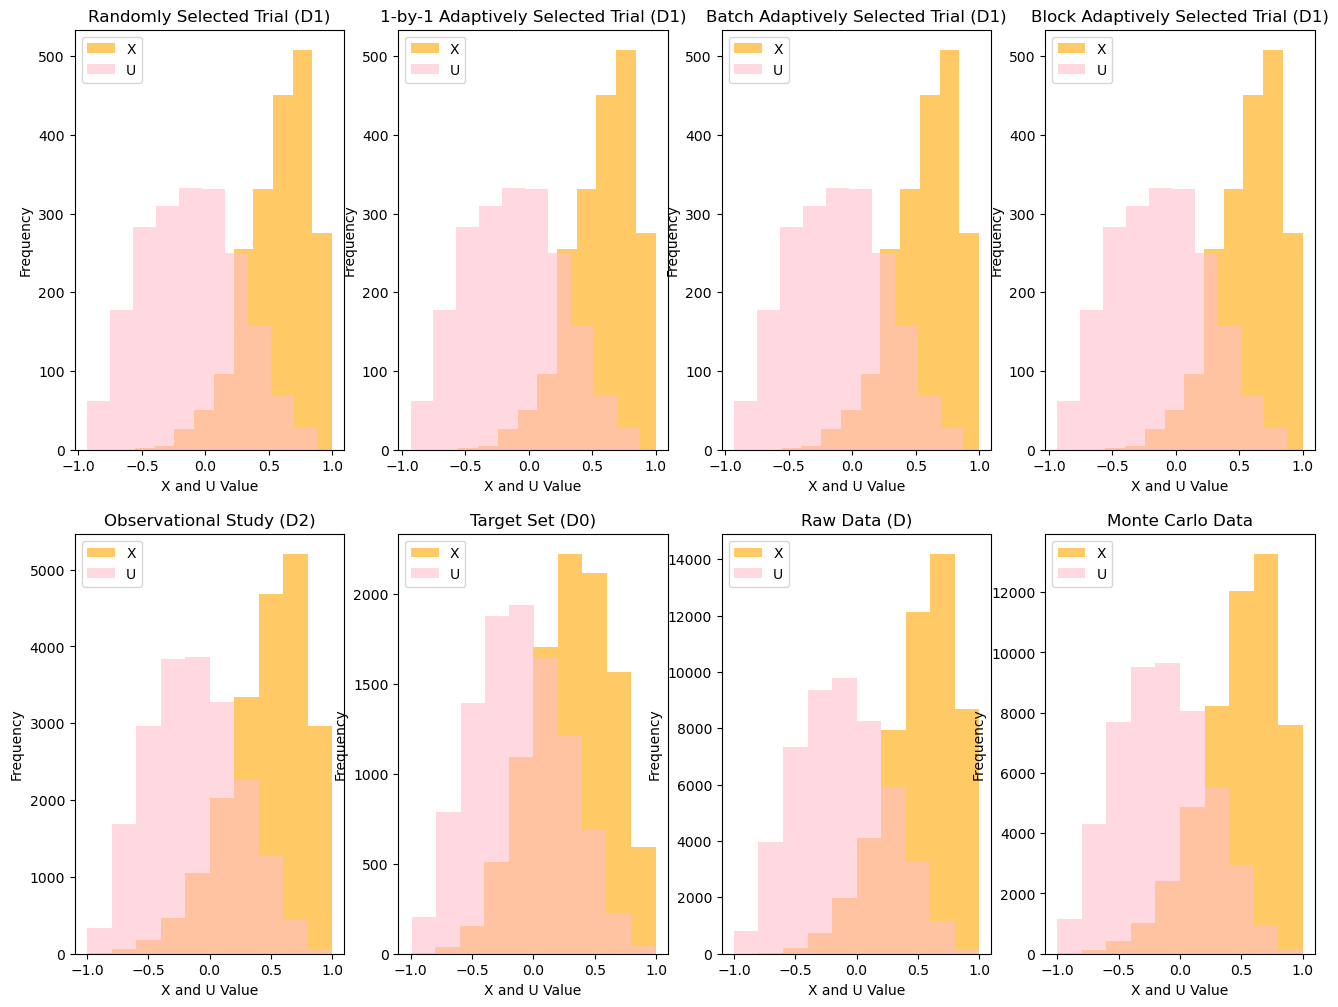
\includegraphics[scale=0.3]{Report/Figure/XvsU.jpg}
    \caption{This figure plots the distributions of the covariate $X$ (orange) and the confounding variable $U$ (pink) across different datasets. In all datasets, both $X$ and $U$ exhibit skewed distributions, reflecting the Beta distributions they are drawn from. The raw data reflects the full population. The Monte Carlo data, generated independently but following the same structure, shows a nearly identical distribution to the raw data. The trial sets consist much lower percentage of lower-valued $X$ than the target set.}
    \label{XvsU}
\end{figure}
\FloatBarrier

\begin{figure}[hbt!]
    \centering
    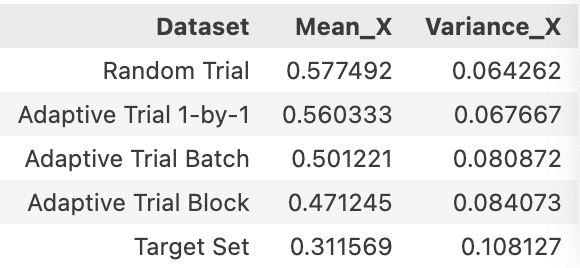
\includegraphics[scale=0.3]{Report/Figure/Xmismatch.jpg}
    \caption{This table shows the mean and variance of covariate $X$ in trial and target sets. Substantial difference exists.}
    \label{Xmismatch}
\end{figure}
\FloatBarrier


\begin{figure}[hbt!]
    \centering
    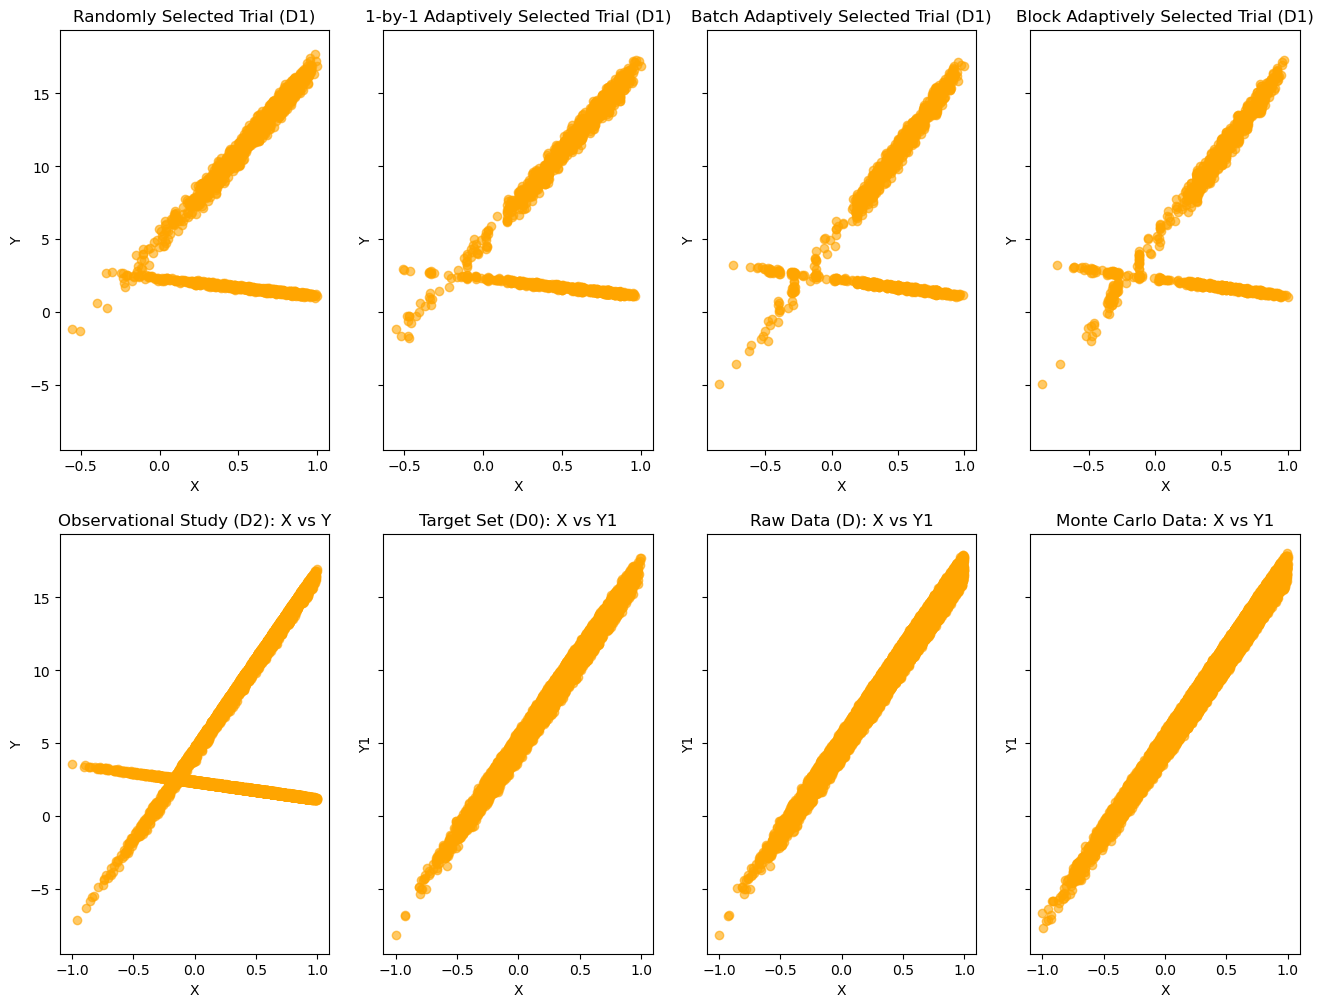
\includegraphics[scale=0.25]{Report/Figure/XvsY.jpg}
    \caption{This figure displays scatter plots of $X$ against $Y$ across all datasets. In the trial sets and observational study, the treatment ($A=1$) and control ($A=0$) groups are clearly separated into two linear bands, indicating the linear outcome models for $Y^1$ and $Y^0$. In the adaptive trials, we observe denser sampling in regions where uncertainty about $Y$ is higher, particularly for intermediate $X$ values. The target set, raw data and Monte Carlo data, which represent the true population outcomes on $Y^1$, show the relationships between $X$ and $Y^1$.}
    \label{XvsY}
\end{figure}
\FloatBarrier
    
\begin{figure}[hbt!]
    \centering
    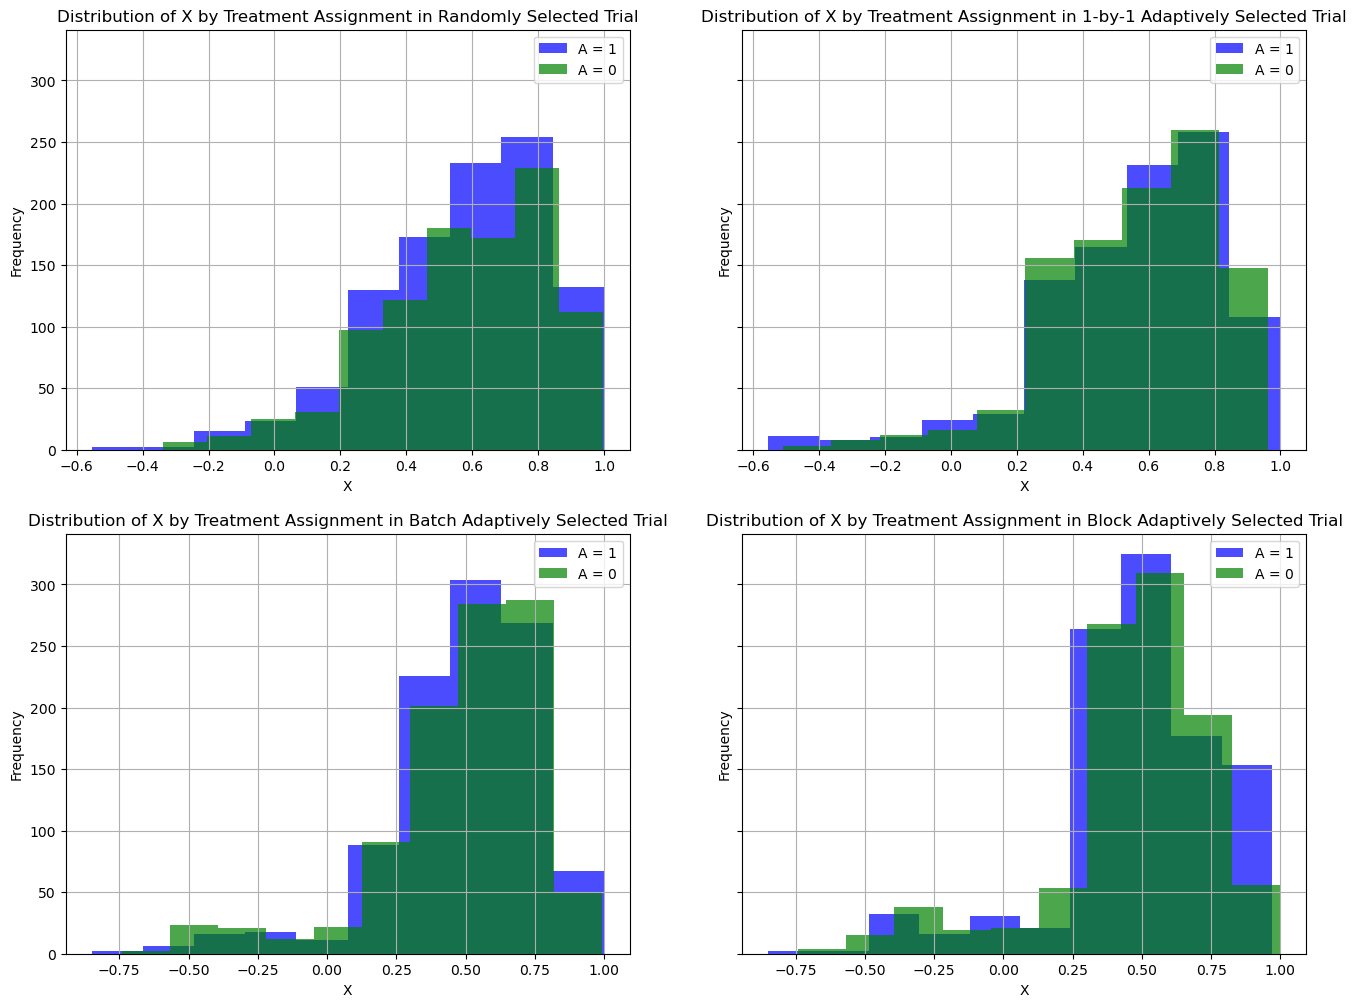
\includegraphics[scale=0.2]{Report/Figure/XinRCT.jpg}
    \caption{This figure plots the distribution of $X$ by treatment assignment ($A=1$ for treatment, $A=0$ for control) in the different trial datasets. For all the trial sets, treatment and control groups exhibit balanced distributions of $X$ (largely overlapped in the green and blue regions), as treatment assignment is random.}
    \label{XinRCT}
\end{figure}
%\FloatBarrier

\begin{figure}[hbt!]
    \centering
    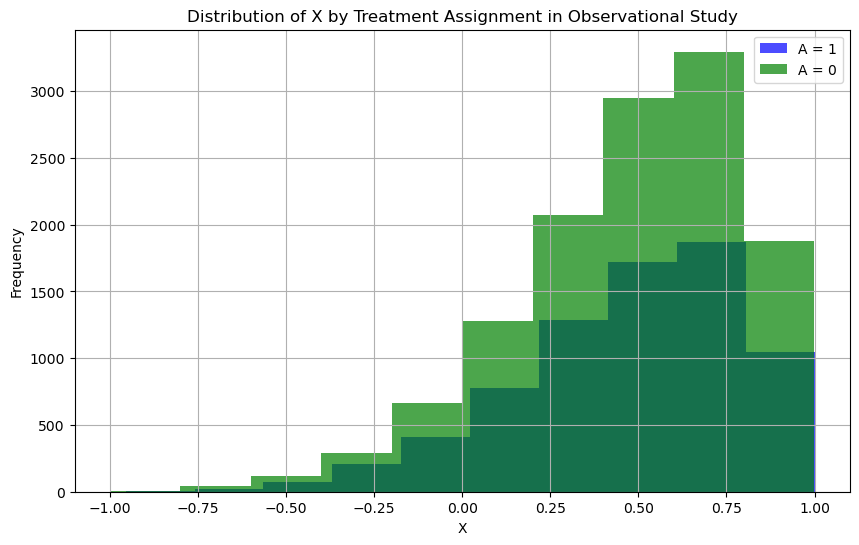
\includegraphics[scale=0.25]{Report/Figure/XinOS.jpg}
    \caption{This figure shows the distribution of $X$ by treatment assignment ($A=1$ for treatment, $A=0$ for control) in the observational study. Unlike the trial sets, where treatment assignment is random, the observational study shows a clear imbalance. Note that we use a logistic model for treatment assignment based on both $X$ and the confounding variable $U$, though $U$ is not plotted in this case.}
    \label{XinOS}
\end{figure}
\FloatBarrier

\begin{figure}[hbt!]
    \centering
    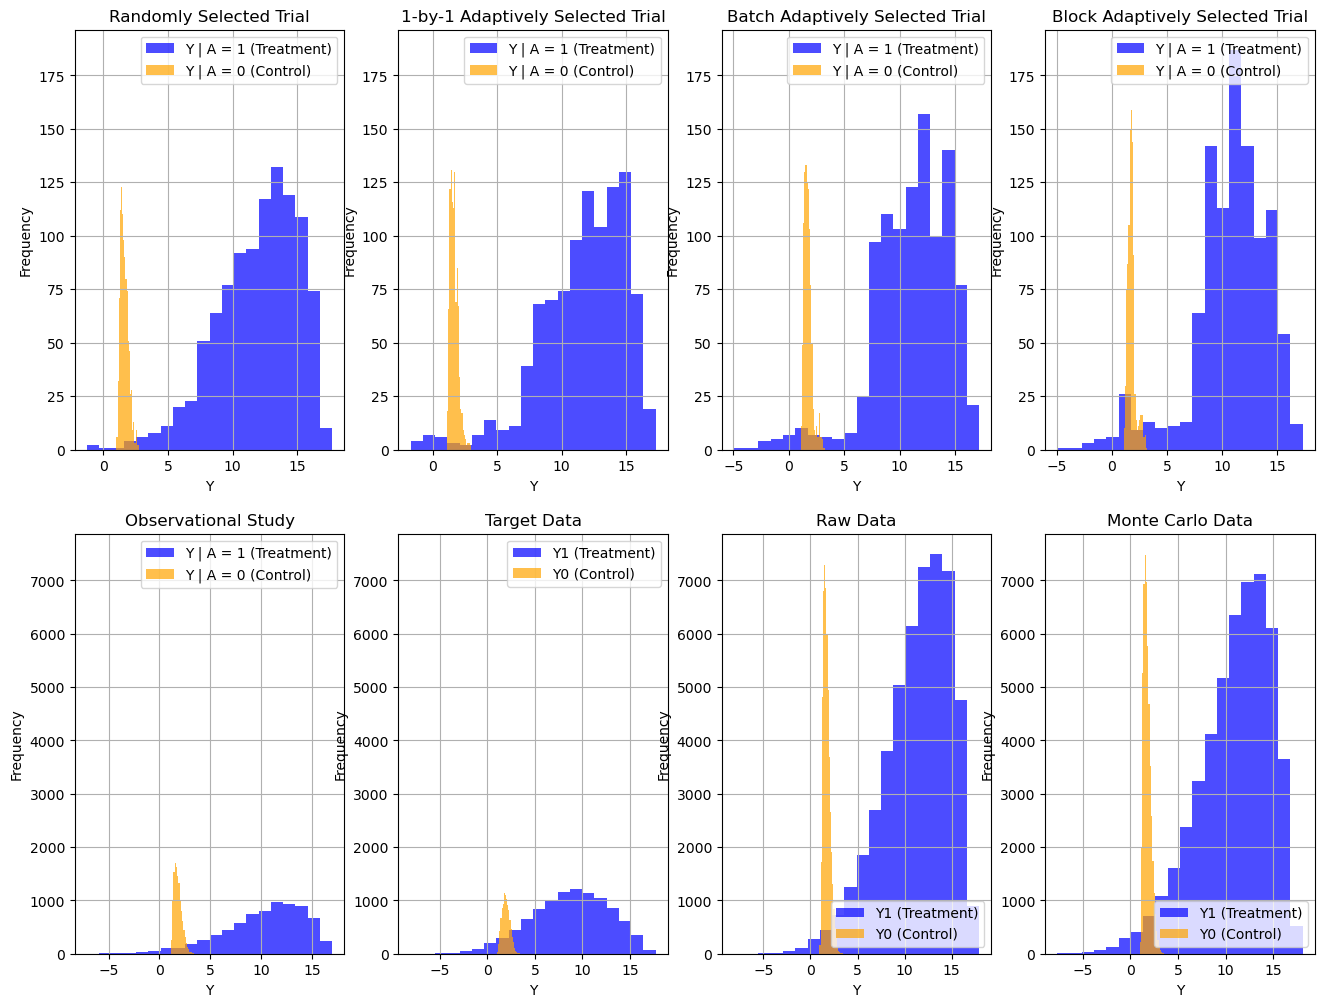
\includegraphics[scale=0.3]{Report/Figure/YvsA.jpg}
    \caption{This figure presents histograms of outcome $Y$ for treatment ($A=1$) and control ($A=0$) groups across all datasets. In the trial sets, the outcomes for $A=1$ and $A=0$ are well separated. Adaptive trials focus sampling on regions with higher uncertainty in $Y$, especially around intermediate $X$ values. The target set, raw data, and Monte Carlo data provide benchmarks for comparison, reflecting the true population outcomes.}
    \label{YvsA}
\end{figure}
\FloatBarrier

Figure \ref{mean_std_results} visualizes the performance of different methods (Baseline models, ABC, and AOM) in terms of the mean and standard deviation of the treatment outcome $Y^1$ as the trial size increases. Our results are evaluated against raw data, Monte Carlo data, and target data. While the error is not directly plotted, it can be inferred from the distance between the estimates of each method and the true mean (represented by the black line). Standard deviations are represented by the spread (dotted lines) around the means. 

\textbf{Variance Trends}: The standard deviations are initially high for small trial sizes but decrease as the trial size increases in Figures \ref{mean_std_results} - \ref{variance}. The standard deviation does not change for baseline 1 approach as trial size changes due to the baseline 1 method not involving trial data at all. The standard deviation for the Baseline 2 method does not significantly decrease as trial size increases, possibly because it relies solely on trial data, which has covariate mismatch with the target data, limiting its ability to capture variability in the broader population. However, this hypothesis remains to be investigated further. Adaptive trial selections demonstrate more efficient variance reduction compared to random selection. By prioritizing informative samples, these methods achieve more rapid reductions in variance as the trial size increases. 

\textbf{Performance of ABC and AOM}: Figures \ref{se_raw} to \ref{se_target} show the SE trends for different methods (Baseline 1, Baseline 2, ABC, and AOM) under varying trial sizes and sampling strategies. Across all cases, AOM and ABC consistently outperform Baseline 1 and Baseline 2 in reducing SE, with Baseline 1 performing the worst (depends solely on OS data). The AOM method shows the most robust performance across all trial sampling approaches, leveraging both trial and observational data effectively. 

\textbf{Impact of Trial Size on Estimation Error}: Baseline 1 is not affected by the change in trial size as it relies solely on the OS data. As trial size increases, all methods except for Baseline 1 show improvement in their mean estimates initially, converging closer to the true mean. However, the rate of improvement stops after the trial size reaches certain point, depending on different trial sampling strategies (e.g. $500$ for Random Sampling, $300$ for 1-by-1 Adaptive Sampling). This indicates that simply increasing the trial size beyond certain point yields diminishing returns in reducing error. The limited improvement in the mean estimates at larger trial sizes is not surprising due to the transportation bias in the covariate $X$ between the trial and target populations. Since transportation bias persists regardless of trial size, further increasing trial size cannot eliminate this source of bias. Moreover, enlarging the trial size may amplify the influence of this mismatch, as more samples from the skewed trial distribution disproportionately reinforce the existing bias, potentially worsening the error beyond a certain point.

\textbf{SE Comparison for Trial Selection Strategies}: We now take a closer look at the different sampling strategies across methods. Figures \ref{se_rct_raw} to \ref{se_rct_target} present the SE for Baseline 1, Baseline 2, ABC, and AOM, focusing on comparing the random sampling and three adaptive trial selection strategies. Adaptive sampling, particularly batch and iterative strategies, generally outperforms random sampling in reducing SE as they reach the "best" result with smaller trial sizes. The "best" SE value achieved by the Adaptive 1-by-1 sampling method is the lowest among all sampling methods. The block adaptive strategy underperforms others in this experiment, achieving the best SE at a bigger trial size. This is expected due to its reliance on the initial random sample, which constitutes $1/3$ of the desired trial size. If this initial sample poorly represents the covariate space, subsequent selections might be less informative. \\

The results evaluated against $S=0$ data in the raw data, Monte Carlo data, and the target set are consistent, with minimal differences across the three standards. This consistency is expected given their construction—Monte Carlo data and raw data are generated using the exact same process, and the target set is a subset of the raw data. Thus, their similarities reflect the controlled and uniform setup of the simulations. 

\begin{figure}[hbt!]
    \centering
    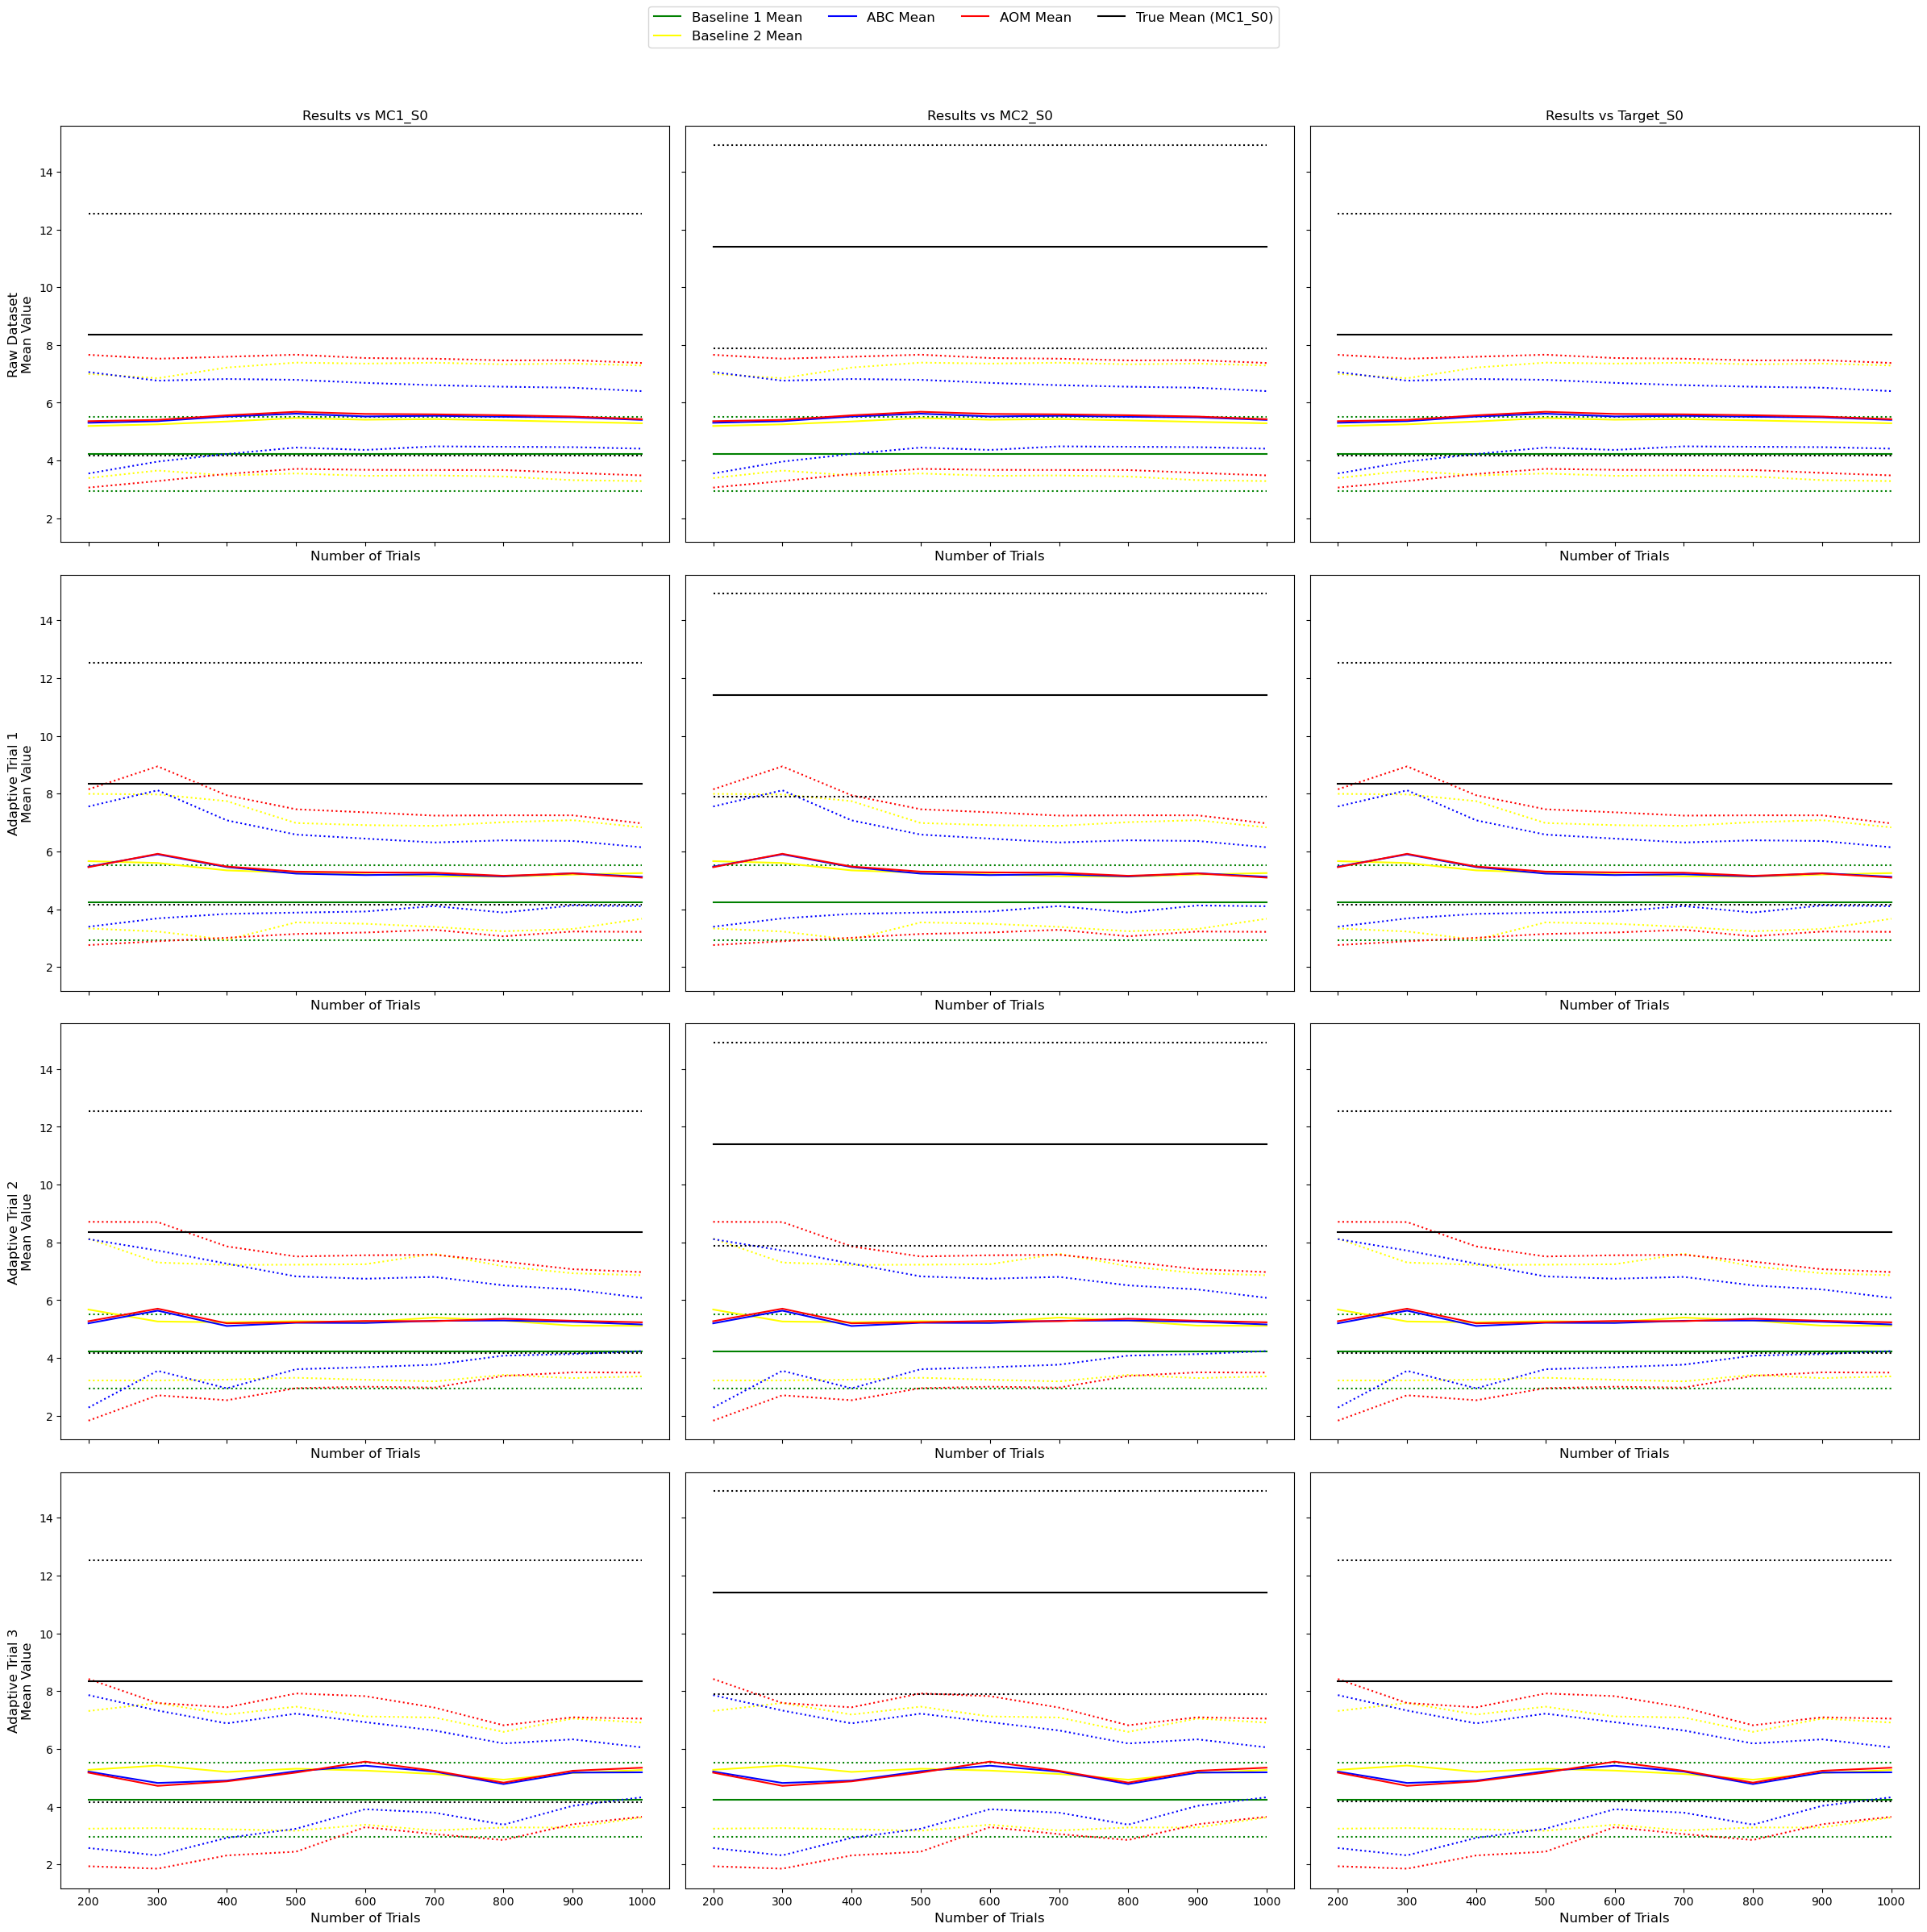
\includegraphics[scale=0.15]{Report/Figure/mean_std_results.jpg}
    \caption{X-Axis: Number of trials (increasing trial sample size). Y-Axis: The mean $\pm$ standard deviation of treatment outcome ($Y^1$). Black Line: Represents the true mean outcome for the target population, serving as the benchmark. $3$ standards are used, represented by $3$ columns of plots. Colored Lines: The mean treatment outcome estimated. Dotted Lines: Represent the standard deviation of each estimate, indicating how spread out the estimated treatment outcomes are. There are two dotted lines below and above the mean for all methods, representing mean $\pm$ standard deviation.}
    \label{mean_std_results}
\end{figure}
\FloatBarrier

\begin{figure}[hbt!]
    \centering
    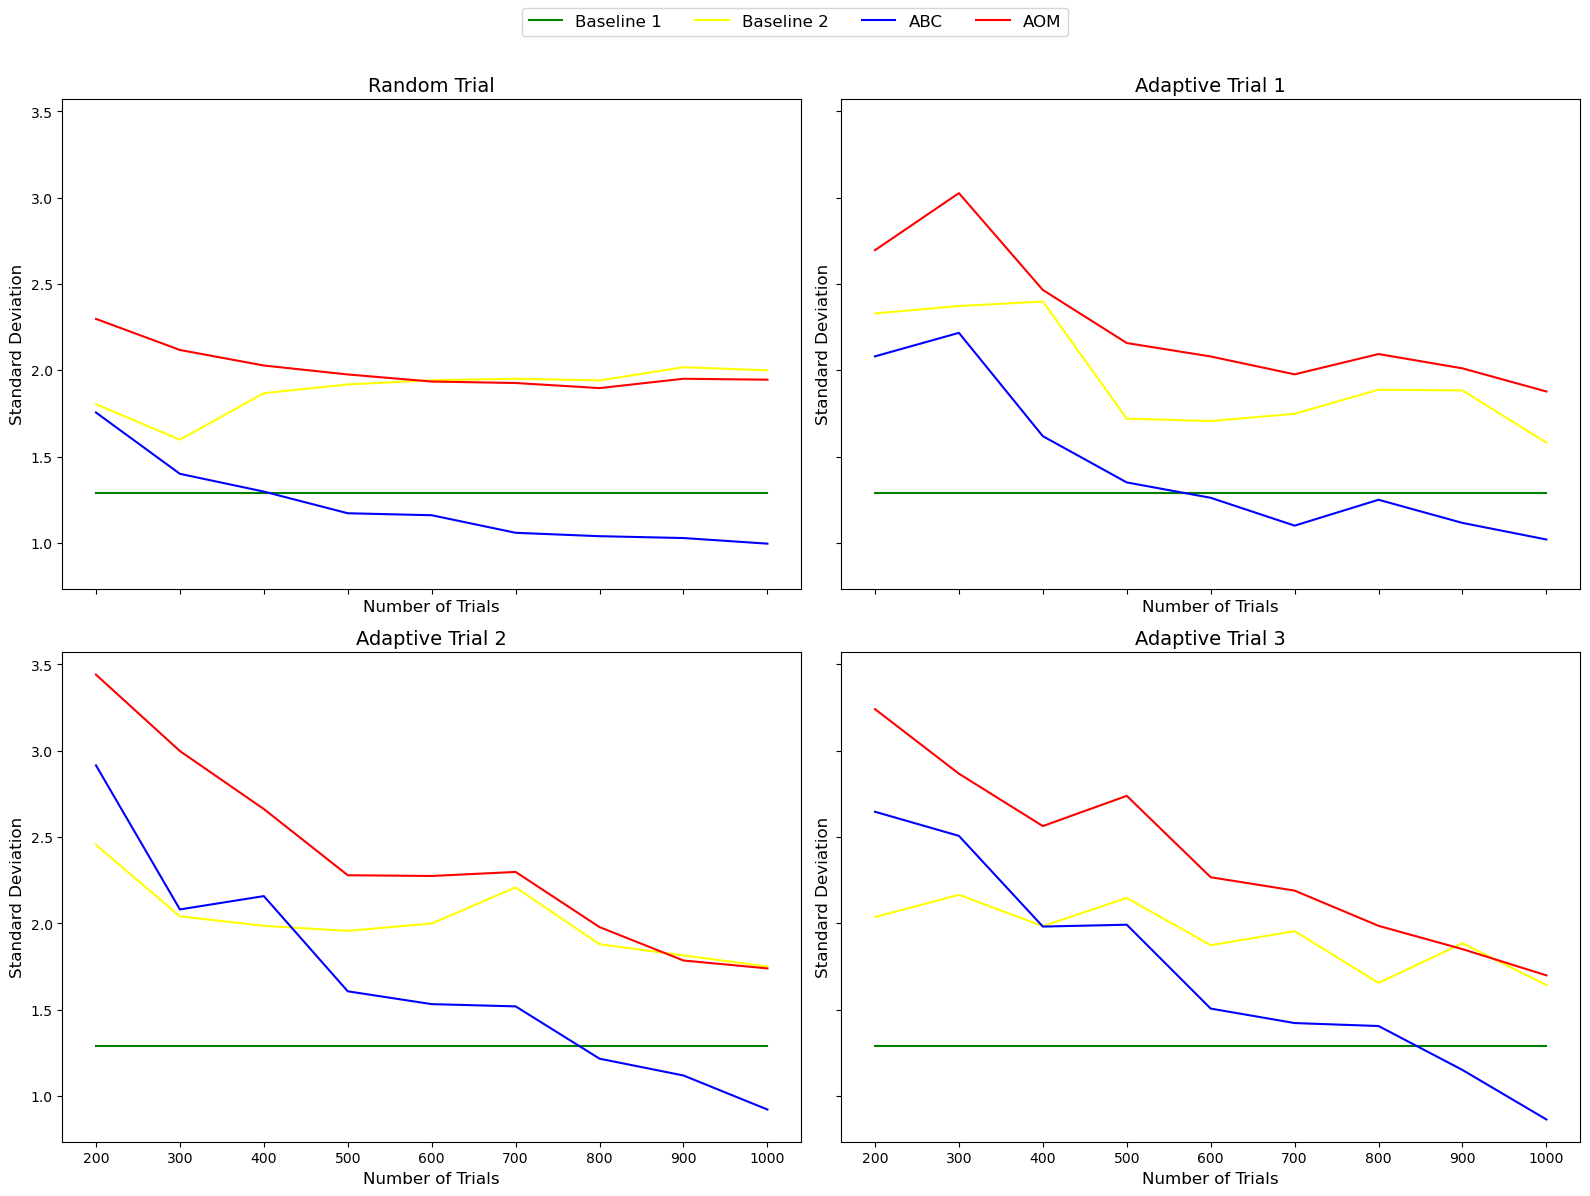
\includegraphics[scale=0.15]{Report/Figure/variance.jpg}
    \caption{X-Axis: Number of trials (increasing trial sample size). Y-Axis: The standard deviartion of estimates on treatment outcome $Y^1$. Colored Lines: different methods (Baseline 1, Baseline 2, ABC, AOM).}
    \label{variance}
\end{figure}
\FloatBarrier


\begin{figure}[hbt!]
    \centering
    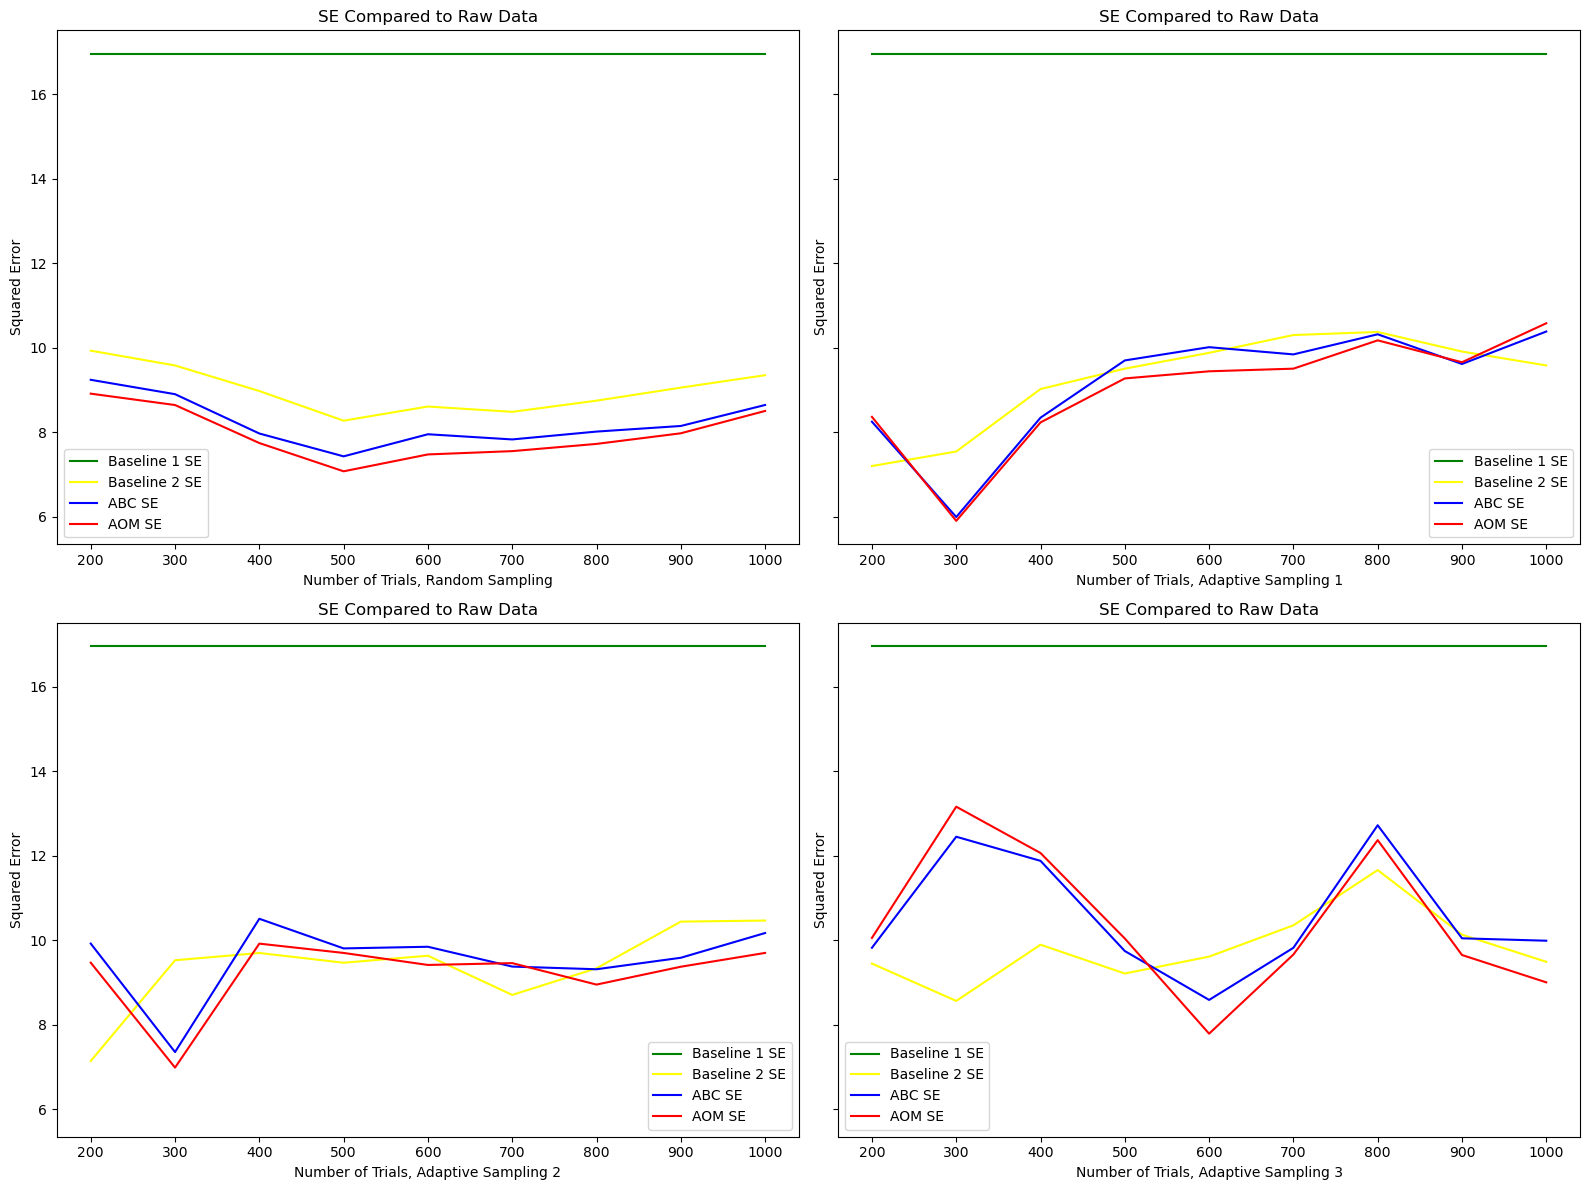
\includegraphics[scale=0.15]{Report/Figure/se_raw.jpg}
    \caption{This plot compares the SE of different methods: Baseline 1, Baseline 2, ABC, and AOM against the average treatment outcome in the $S = 0$ subset from the raw data. The x-axis represents the number of trials, while the y-axis indicates the SE. The plot includes results for random sampling trial (top left) and adaptive sampling trials (top right for 1-by-1, bottom left for batch, and bottom right for block).}
    \label{se_raw}
\end{figure}
\FloatBarrier

\begin{figure}[hbt!]
    \centering
    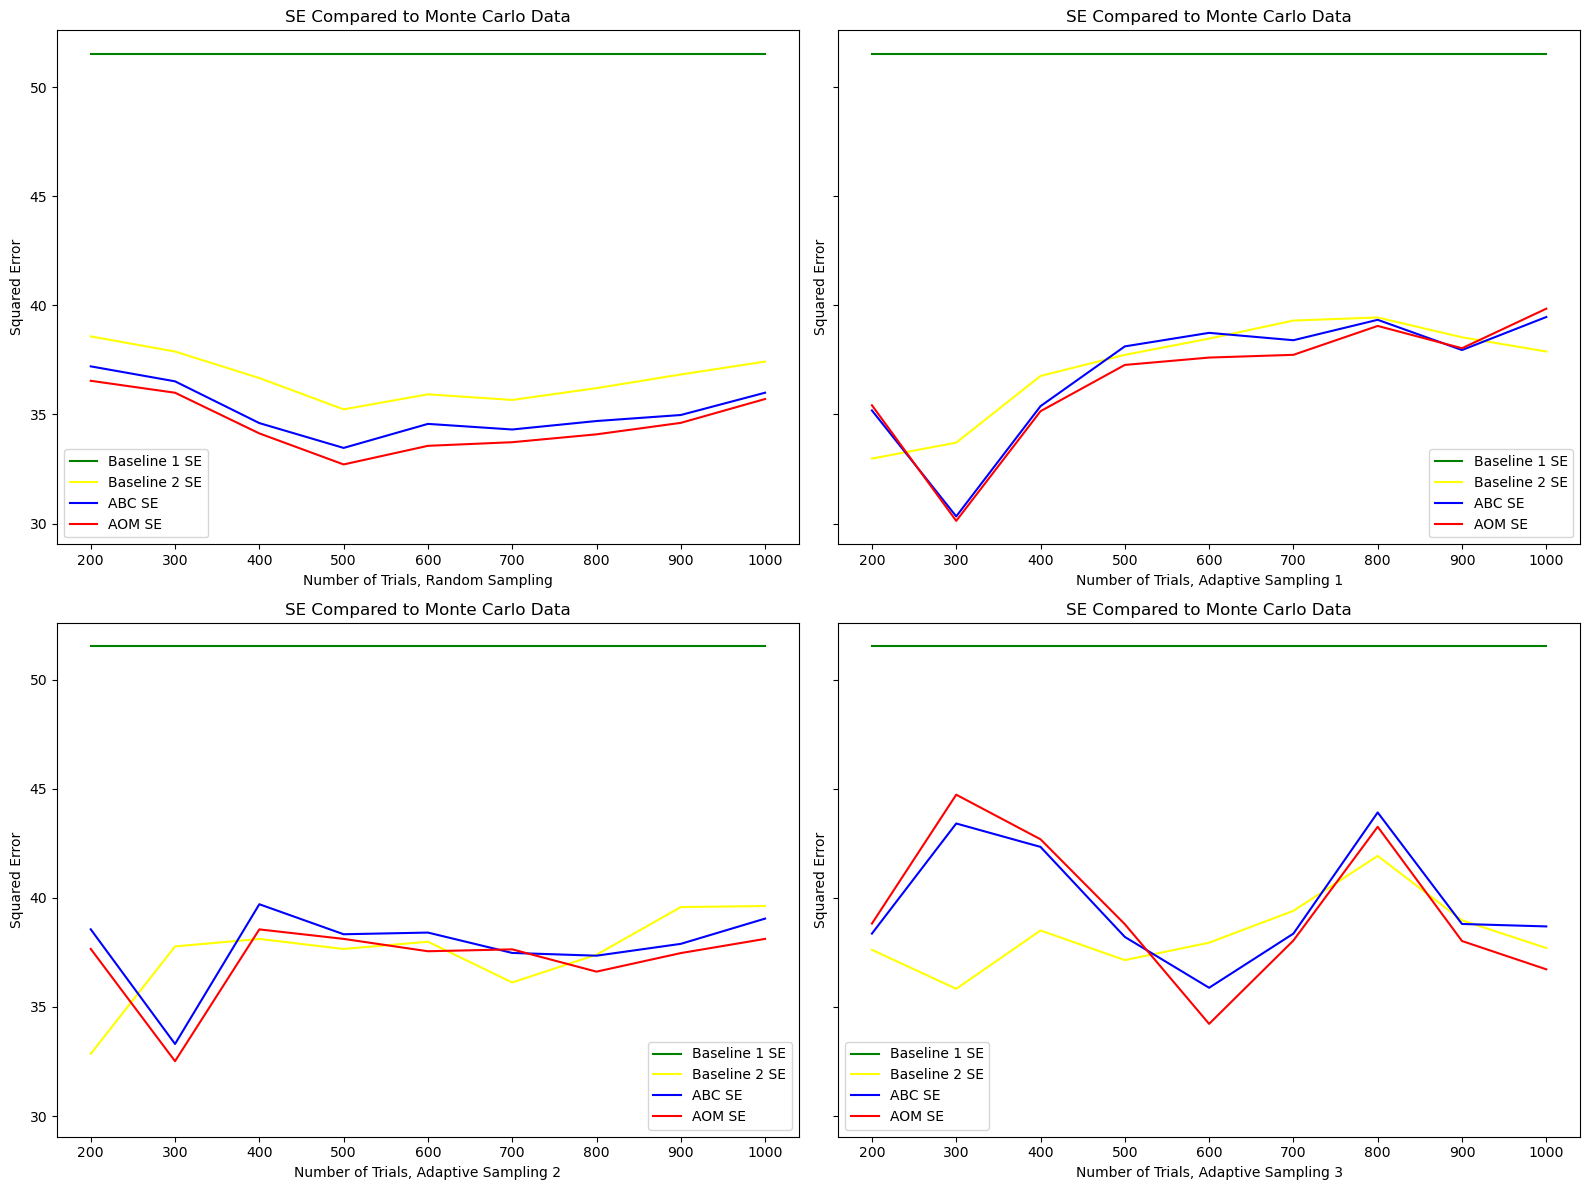
\includegraphics[scale=0.15]{Report/Figure/se_mc.jpg}
    \caption{This plot compares the SE of different methods: Baseline 1, Baseline 2, ABC, and AOM against the average treatment outcome in the Monte Carlo $S=0$ data. The x-axis represents the number of trials, while the y-axis indicates the SE. The plot includes results for random sampling trial (top left) and adaptive sampling trials (top right for 1-by-1, bottom left for batch, and bottom right for block).}
    \label{se_mc}
\end{figure}
\FloatBarrier

\begin{figure}[hbt!]
    \centering
    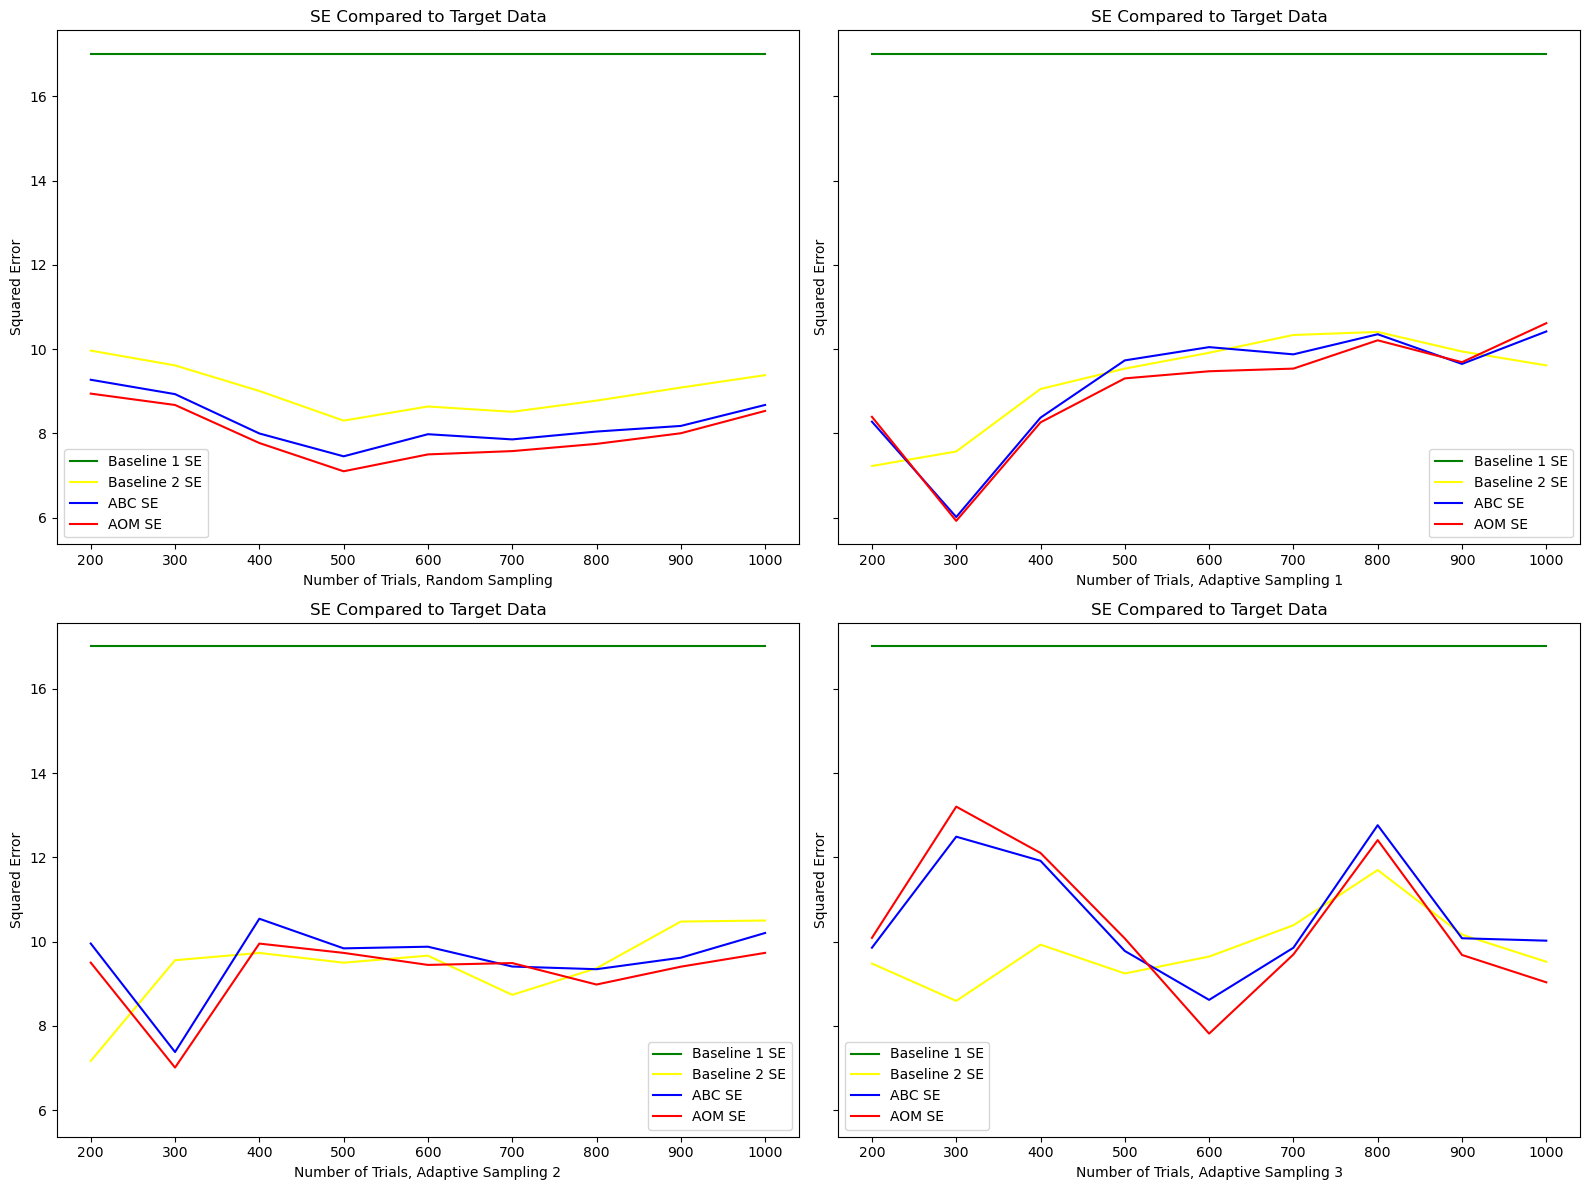
\includegraphics[scale=0.15]{Report/Figure/se_target.jpg}
    \caption{This plot compares the SE of different methods: Baseline 1, Baseline 2, ABC, and AOM against the average treatment outcome in target set $D_0$. The x-axis represents the number of trials, while the y-axis indicates the SE. The plot includes results for random sampling trial (top left) and adaptive sampling trials (top right for 1-by-1, bottom left for batch, and bottom right for block).}
    \label{se_target}
\end{figure}
\FloatBarrier

\begin{figure}[hbt!]
    \centering
    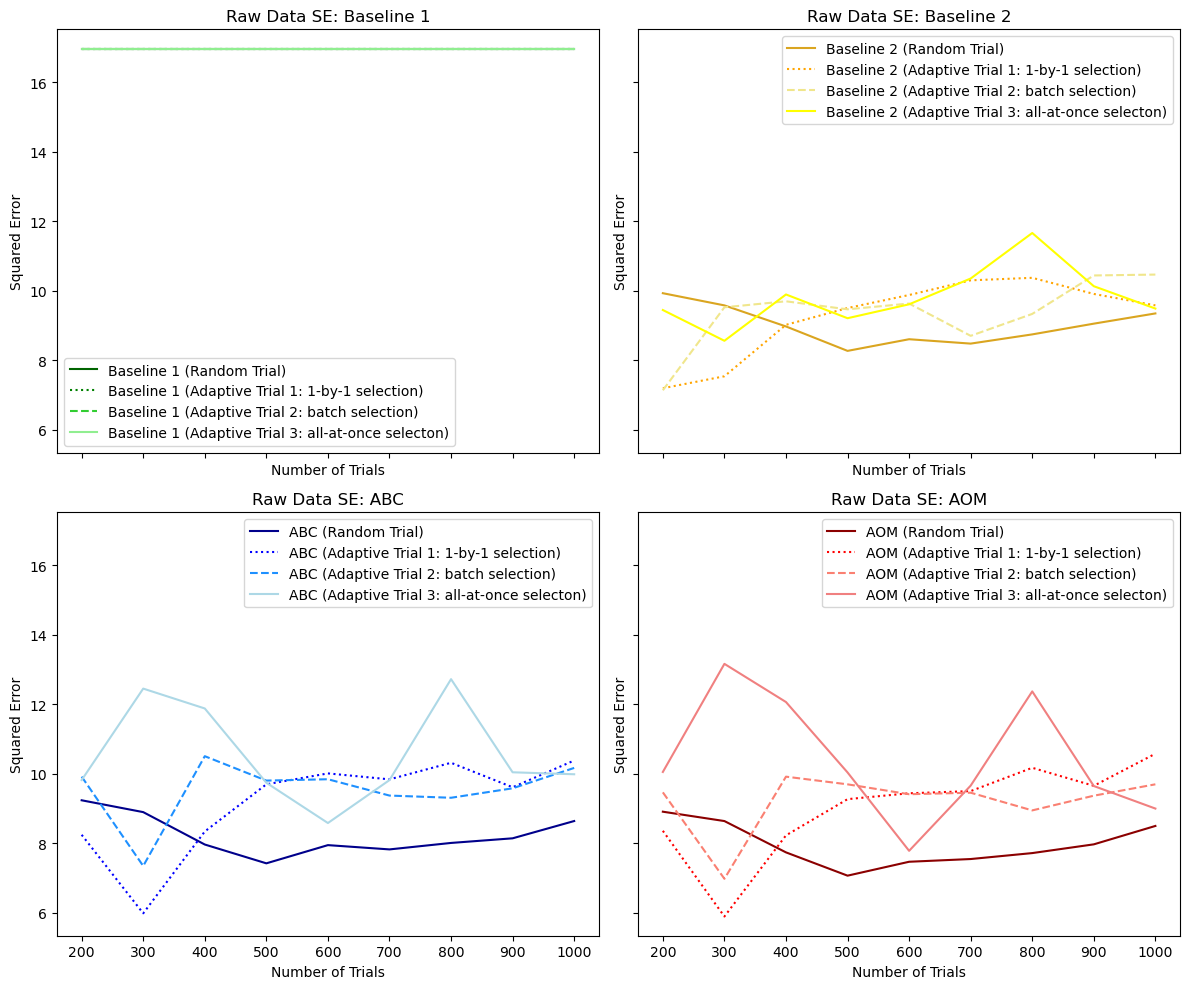
\includegraphics[scale=0.2]{Report/Figure/se_rct_raw.jpg}
    \caption{This plot compares the SE of different trial sampling strategies. The SE is calculated against the average outcome in $S=0$ subset of raw data $D$. The x-axis represents the number of trials, while the y-axis indicates the SE.}
    \label{se_rct_raw}
\end{figure}
\FloatBarrier

\begin{figure}[hbt!]
    \centering
    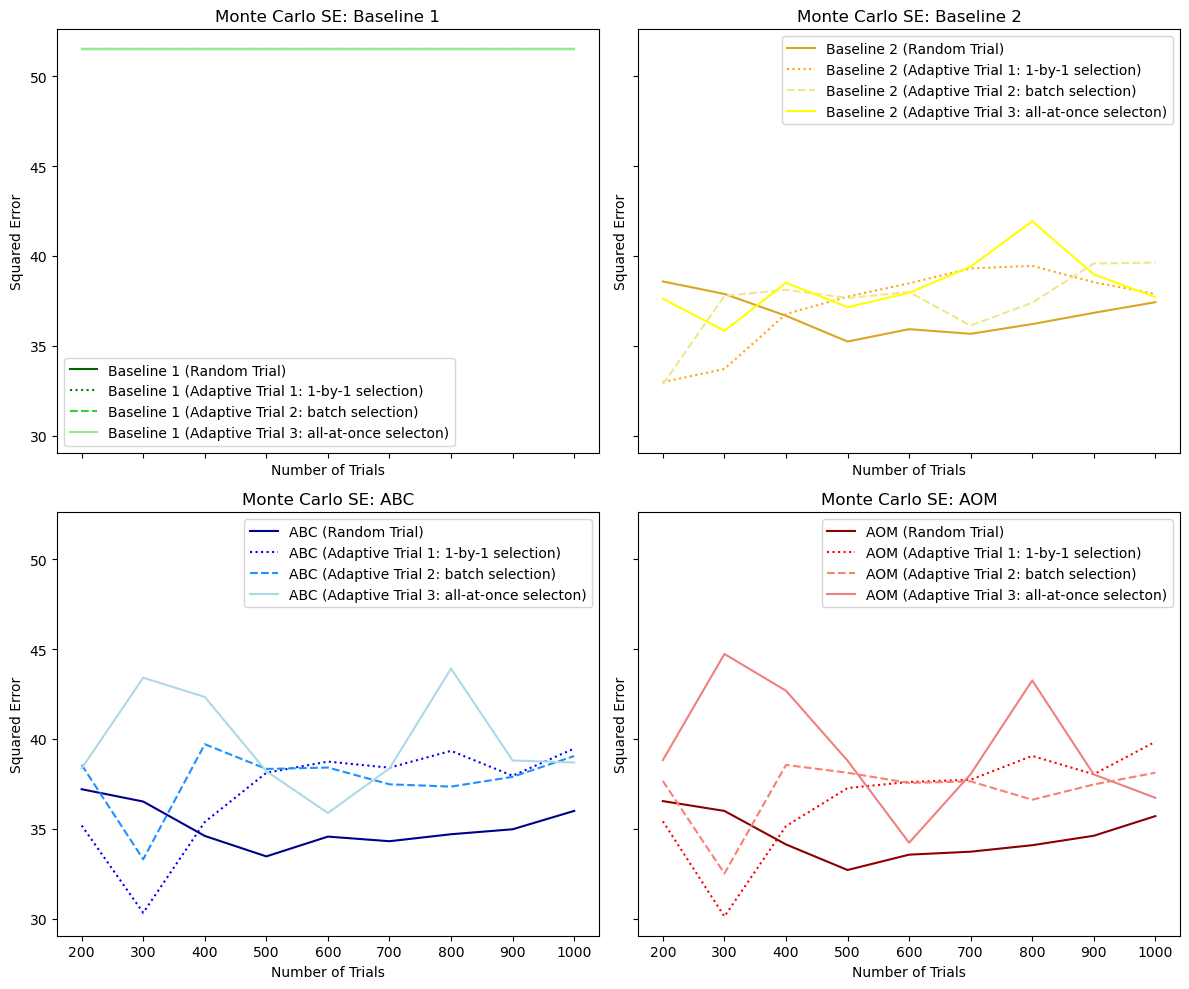
\includegraphics[scale=0.2]{Report/Figure/se_rct_mc.jpg}
    \caption{This plot compares the SE of different trial sampling strategies. The SE is calculated against the average outcome in $S=0$ subset of Monte Carlo data. The x-axis represents the number of trials, while the y-axis indicates the SE.}
    \label{se_rct_mc}
\end{figure}
\FloatBarrier

\begin{figure}[hbt!]
    \centering
    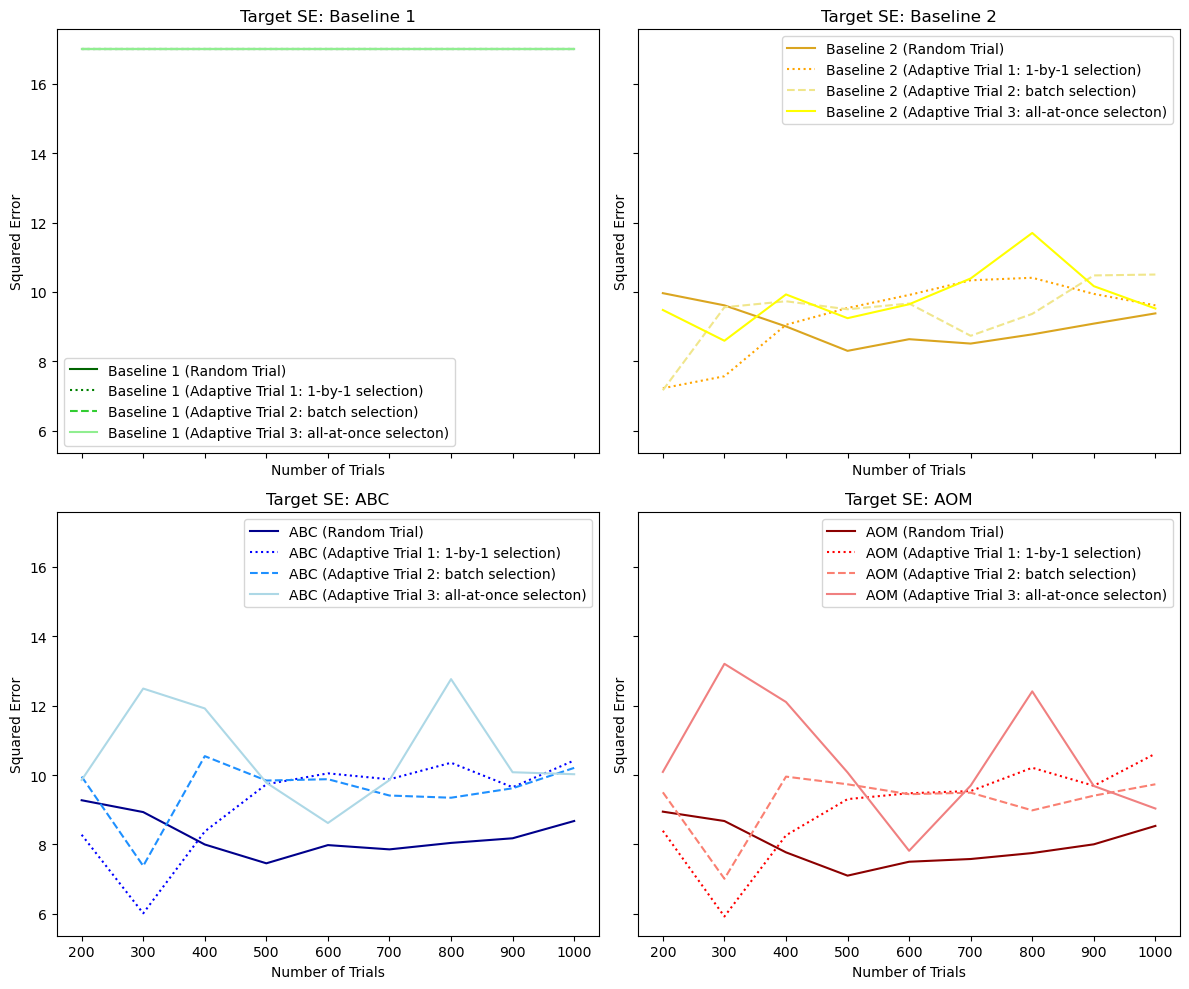
\includegraphics[scale=0.2]{Report/Figure/se_rct_target.jpg}
    \caption{This plot compares the SE of different trial sampling strategies. The SE is calculated against the average outcome in the target set $D_0$. The x-axis represents the number of trials, while the y-axis indicates the SE.}
    \label{se_rct_target}
\end{figure}
\FloatBarrier


\subsection{Study Summary and Discussion}
In summary, we investigated whether the PPCI framework works under mismatched covariate between the trial and target sets. The results confirm that PPCI remains effective, with ABC and AOM outperforming the baselines, though the improvements are less pronounced compared to the no-mismatch case as shown in the original paper \citep{qp}. Adaptive sampling strategies in the trial set show certain enhancement on estimation accuracy. When a mismatch exists, the SE reduction levels off beyond a certain number of trials, indicating diminishing returns afterwards. This suggests that increasing trial size alone cannot resolve inherent mismatches in this case.\\

A key limitation of our study is that performance metrics are based on squared error (SE) from a single run for each fixed trial size. Without multiple runs at fixed trial sizes, the results may lack stability and be more influenced by the randomness of a single simulation. Calculating the mean squared error (MSE) through multiple runs would provide a more robust and reliable measure of estimator performance. However, to maintain computational feasibility and focus as an initial exploratory study, we limited the scope to single-run evaluations for each trial size. Future work could also explore alternative error metrics, such as absolute error or confidence interval coverage, to provide a more nuanced evaluation of estimator performance. \\

For future research, it would be valuable to extend the analysis to include different average outcomes such as $\mathbb{E}[Y^0]$, and the treatment effect $\mathbb{E}[Y^1] - \mathbb{E}[Y^0]$, to provide a more comprehensive assessment of causal effects. Additionally, experiments could be expanded into cases where the covariate distributions are entirely different, such as in unnested experimental setups, or by introducing more covariates with varying complexities and interaction effects to simulate realistic scenarios. Exploring target distributions drawn from more complex structures, such as multimodal or heavy-tailed distributions, could better reflect heterogeneous populations. Dynamic trial participation probabilities dependent on multiple covariates would further enhance the framework's generalizability. Finally, applying PPCI to real-world datasets would provide critical insights into its practical utility and robustness.
\clearpage
\printbibliography
\end{document}
